%Your one page proposal should explicitly specify a title, the names of members of your group, the
%problem or question that your project addresses, the hypothesis that is being tested, the network 
%architecture and learning method(s) you will evaluate, the motivations for the evaluation, the 
%implementation language, the nature and source of the training data, and the evaluation design
%Your final report should include the same information, a tabulation of results, a discussion stating 
%your conclusions, and a short appendix with a sample run for each method you evaluate. Program 
%listings of software that you create are to be submitted separately

\documentclass{acm_proc_article-sp}
\usepackage[usenames,dvipsnames]{xcolor}
\usepackage{hyperref}

\newcommand{\todo}[1]{\textcolor{orange}{\textbf{TODO}: #1}} %~\\ 
\newcommand{\unsure}[1]{\textcolor{Mulberry}{\textbf{?} #1 \textbf{?}}}
\newcommand{\brainstorm}[1]{\textcolor{ProcessBlue}{\textbf{Brainstorming}: #1}}
\def\bs{\brainstorm}
\newcommand{\wordchoice}[1]{\textcolor{red}{\textbf{#1}}}
\def\wc{\wordchoice}

\begin{document}

\title{Comparing Performances of Recurrent Jordan and Elman Neural Networks}
\numberofauthors{2}
\author{
\alignauthor James Parker\\%\titlenote{Dr.~Trovato insisted his name be first.}\\
       \affaddr{Department of Computer Science}\\
       \affaddr{University of Maryland, College Park}\\
       \affaddr{College Park, MD}\\
       \email{jp@jamesparker.me}
\alignauthor Kerry Cheng\\%\titlenote{Dr.~Trovato insisted his name be first.}\\
       \affaddr{Department of Computer Science}\\
       \affaddr{University of Maryland, College Park}\\
       \affaddr{College Park, MD}\\
       \email{kerry.cheng.2013@gmail.com}
}

\maketitle

\begin{abstract}
\todo{overview of entire paper, including results}
\end{abstract}
\section{Introduction} % problem, solution, your contribution, outline
Jordan and Elman networks are two forms of recurrent neural networks that share very similar behavior and functionality. 
They are both used to perform pattern recognition and time series forecasting given data over time. 
Jordan networks were first introduced by Jordan with the novel approach that the output of a neural network could be copied back to a new context layer in the network \cite{jordan}. Then the network could learn the associated weights of this new context layer by standard back propagation. 
Elman expanded on this idea by introducing Elman networks \cite{elman}. 
The difference with this new type of network is that the hidden layer is copied back to the context layer, instead of the output layer. 
Both of these networks seems to have a similar flavor in their approaches.
The problem is that there does not currently seem to be any detailed comparison on the performance of these two neural networks that covers many data sets. 

To fix this problem, we set out to perform a detailed comparison between Jordan and Elman recurrent neural networks. 
We began by implementing both network in the new programming language, Julia. 
We then train both types of networks on time varying input and output data while tuning training parameters to get best results. 
We chose five separate data sets to evaluate on, which all originate from the Matlab Neural Network Toolbox Sample Data Sets \cite{data}. 
These data sets were used to predict both continuous and discrete types of outputs.

This paper is laid out as follows. First we discuss our motivation for comparing Jordan and Elman networks in Julia. %for implementing Jordan and Elman networks in Julia
Then we cover the methods of our comparison, as well as the data sets used in our comparison. The next section goes over our results. Finally we discuss our results and draw conclusions.

\section{Motivation}
We decided to study Elman and Jordan networks because they are both standard techniques to perform training over time varying data. 
We are interested to see which network performs better, even though they take very similar approaches. 
Our hypothesis is that Elman networks should have higher performance than Jordan networks because intuitively, it seems like hidden layers contain more information than output layers. Since the context layers of Elman networks update from the hidden layer rather than the output layer, we expect the Elman networks to perform better. 

We also decided to implement these networks in Julia because it is a relatively new language that shows much potential for technical computing. 
For instance, it has features such as a rich type system and a JIT compiler \cite{julia}. 
Stronger types can help a programmer write more correct and less buggy code. 
The JIT compiler also offers huge speed improvements over interpretted languages like Matlab and R. 
For instance, quicksort in Julia is 105.09 times faster than Matlab's quicksort and is 517.34 times faster than R's quicksort. 
This is possible because instructions are compiled to machine operations instead of being evaluated within another language's interpretter.
Since the language is new, there are a limited number of packages available. Therefore our implementations may actually make an impact and be included as a standard Julia package. 

\begin{figure}
\begin{center}
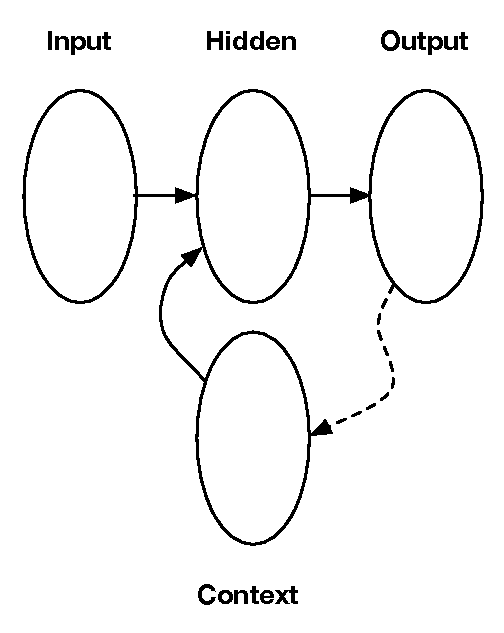
\includegraphics[scale=.8]{Images/jordan.pdf}
\caption{The architecture of a Jordan network.}
\label{fig:jordan}
\end{center}
\end{figure}

\begin{figure}
\begin{center}
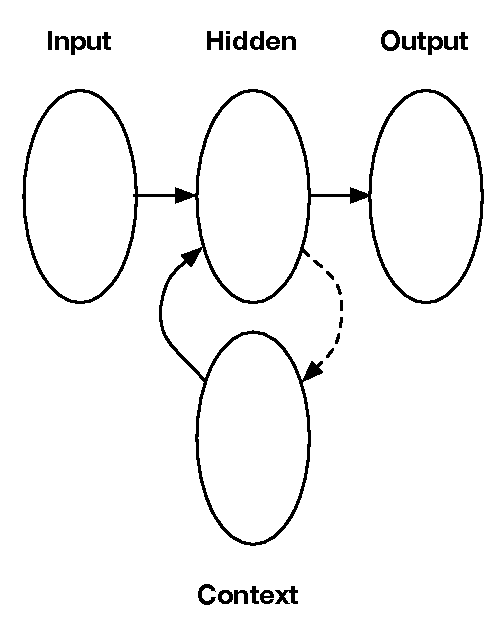
\includegraphics[scale=.8]{Images/elman.pdf}
\caption{The architecture of an Elman network.}
\label{fig:elman}
\end{center}
\end{figure}

\section{Methods}
\todo{network architecture - image, default use logistic/sigmoid activation, add a bias node to the input layer, discuss I/O data types?}
\todo{nature and source of the training data - neural network }
.. 


\section{Results}

\section{Discussion}

... There are a few other that have looked at these two networks???


\bibliographystyle{plain}
\bibliography{myrefs.bib}

\end{document}